\subsection{Predicción del tamaño óptimo de partícula}

Como ya ha sido mencionado a lo largo de esta tesis, el criterio de carga rápida
está definido por la obtención del 80\% de la capacidad del electrodo en 15 
minutos, lo cual se traduce en un SOC$_{\max}$ de 0.8 y una C-rate de 4 C. La
Figura \ref{fig:prediccion} muestra donde se encuentra cada sistema analizado en
el diagrama $\log(\Xi)$--$\log(\ell)$ para dicha C-rate. También se presenta una
curva de nivel con una línea roja correspondiente a SOC$_{\max} = 0.8$. Puede
observarse que tres de los materiales ya se encuentran en la región de 
SOC$_{\max}$ mayor a 0.8 (LCO, LMNO y LNMO), mientras que los otros se encuentran
por debajo de este valor (NG, LTO y LFP).
\begin{figure}[h!]
    \centering
    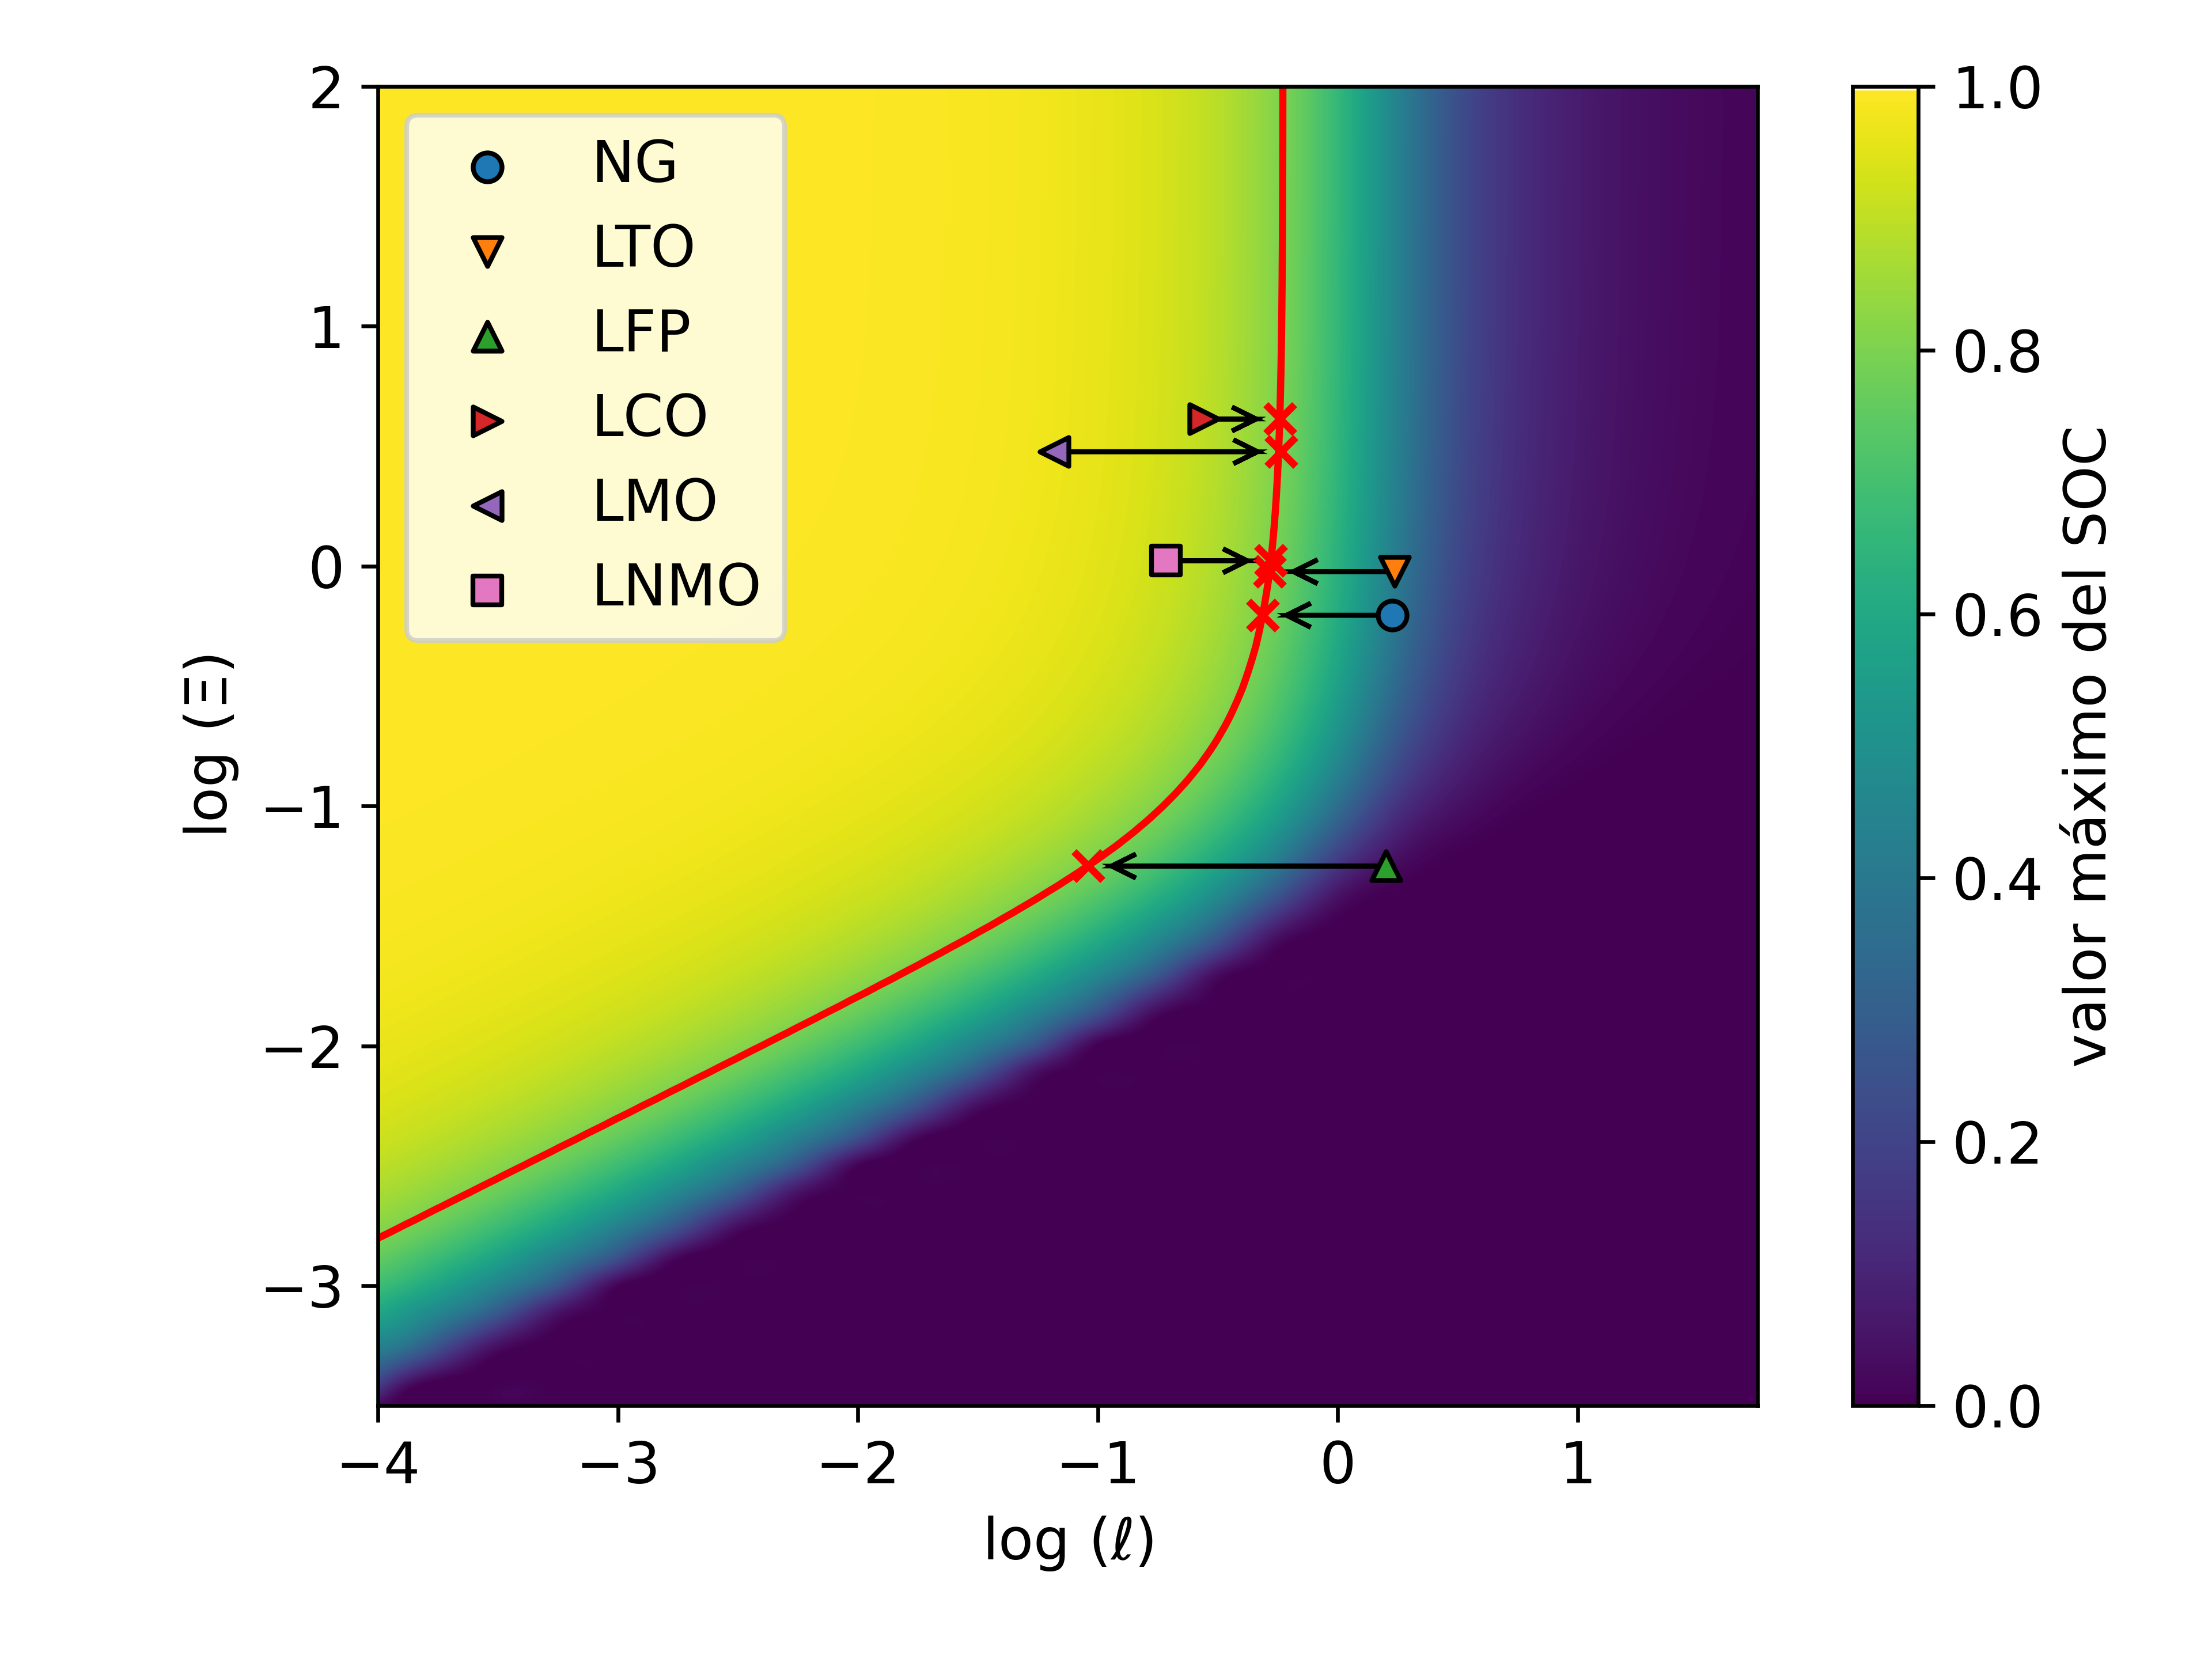
\includegraphics[width=0.7\textwidth]{FastCharging/un/resultados/prediccion/prediccion.png}
    \caption{Diagrama de SOC$_{\max}$ mostrando la ubicación de los materiales 
    usuales de LIBs a 4 C para las referencias consideradas \cite{mancini2022,
    he2012, lei2015, wang2019high, bak2011, nishikawa2017}. En los casos en los 
    que la curva de cargado a 4 C no estaba disponible, el valor del punto fue 
    predicho con el modelo. La línea roja muestra la curva de nivel 
    correspondiente al valor 0.8 de SOC$_{\max}$. Las flechas muestran el cambio
    en el tamaño de la partícula que debería efectuarse para obtener dicho valor
    a la C-rate dada. Las cruces sobre la línea muestran la posición de estos
    tamaños de partícula nuevos.}
    \label{fig:prediccion}
\end{figure}
Haciendo uso del diagrama se puede predecir de una forma simple y rápida el tamaño 
de partícula requerido para satisfacer el criterio de carga rápida. Dado que los
valores de $D$ y $k^0$ ya fueron ajustados
y que el de C-rate está dado por el criterio elegido ($C_r = 4$ C), el valor de $\Xi$ es constante. Luego,
para alcanzar el valor de 0.8 de SOC$_{\max}$ hay que variar $\ell$ y esto se
logra disminuyendo o aumentando el tamaño de la partícula, según sea necesario (ver ecuación \ref{eq:ele}).
Este desplazamiento necesario está representado por las flechas en la Figura 
\ref{fig:prediccion} para cada caso. Ya se ha apreciado que tres sistemas se 
encuentran en la región optimizada (LCO, LMO y LNMO), por lo que en estos casos
los tamaños predichos para alcanzar SOC$_{\max} = 0.8$ a 4 C serán mayores que 
los experimentales. Por el contrario, el resto de los materiales (NG, LTO y LFP) 
tienen que ser mejorados con una reducción del tamaño de partícula
para cumplir la condición. En la tercera columna de la Tabla \ref{t:prediccion} 
se reportan los tamaños de partícula predichos para todos los materiales, que son necesarios para lograr SOC$_{\max} = 0.8$ a $C_r = 4$ C. 
Las incertidumbres se determinaron por propagación de errores con 
derivadas parciales, ya que el tamaño de la partícula sólo aparece en el parámetro
$\ell$, al definir $\ell_{\text{opt}}$ como el valor al cual el SOC$_{\max}$ 
alcanza el valor deseado de 0.8 y usar que $V/A = d/z$ se puede despejar de la 
ecuación \ref{eq:ele} que
\begin{equation}
    d = \sqrt{\frac{t_h z D 10^{\ell_{\text{opt}}}}{C_r}}.
\end{equation}
Si además se supone que toda la incertidumbre está asociada al coeficiente de 
difusión $D$, al cual ya se le calculó su incerteza, se puede obtener que
\begin{equation}
    \Delta d = \frac{1}{2} \sqrt{\frac{t_h z 10^{\ell_{\text{opt}}}}{C_r D}} \Delta D.
\end{equation}

\begin{table}[t]
    \centering
    \caption{Tamaño de partícula experimental y valores predichos para cargar el 80\% del
    electrodo en 15 y 5 minutos.} 
    \setlength\extrarowheight{2pt}\stackon{%
    \begin{tabular}{l c c c}
        \toprule
        \textbf{Material del} &
        \textbf{Tamaño} &  
        \textbf{Tamaño predicho} & 
        \textbf{Tamaño predicho} \\
        \textbf{electrodo} & 
        \textbf{experimental [$\mu$m]} &  
        \textbf{para 15 minutos [$\mu$m]} & 
        \textbf{para 5 minutos [$\mu$m]} \\
        \midrule
        NG & 7.5 & 4.027 $\pm$ 0.002 & 2.167 $\pm$ 0.001 \\
        LTO & 1.75 & 0.962 $\pm$ 0.004 & 0.530 $\pm$ 0.002 \\
        LFP & 0.35 & 0.084 $\pm$ 0.002 & 0.0309 $\pm$ 0.0006 \\
        LCO & 20 & 28.8 $\pm$ 0.6 & 16.4 $\pm$ 0.4 \\
        LMO & 0.025 & 0.0734 $\pm$ 0.0003 & 0.0418 $\pm$ 0.0002 \\
        LNMO & 7.999 & 13 $\pm$ 2 & 7.3 $\pm$ 0.8 \\
        \bottomrule
    \end{tabular}
    }{}
    \label{t:prediccion}
\end{table}

Al observarse un buen desempeño para la carga de 15 minutos, se puede exigir un 
poco más que este criterio y predecir el tamaño de partícula requerido para una
C-rate más alta, por ejemplo, 80\% de la carga en 5 minutos (12 C). Si bien este 
criterio puede parecer sobredemandante a primera vista, reportes recientes consideran 
protocolos de carga de 10 minutos \cite{mattis2021, attia2020}. Los resultados
se muestran en la última columna de la Tabla \ref{t:prediccion}. Como puede 
observarse, el comportamiento depende del sistema y del experimento en particular
considerado. El único caso donde se cumple este último criterio de carga rápida 
es el LMO, ya que el tamaño experimental sobrecumple el criterio. Aunque el LCO 
y el LNMO no cumplen con esto último, las mejoras requeridas en sus tamaños son
menores. En el resto de 
los casos, para el LFP se necesitaría una disminución de un orden de magnitud 
en su tamaño, mientras que para el NG o el LTO se requeriría una
disminución de su tamaño en un factor de 3.
